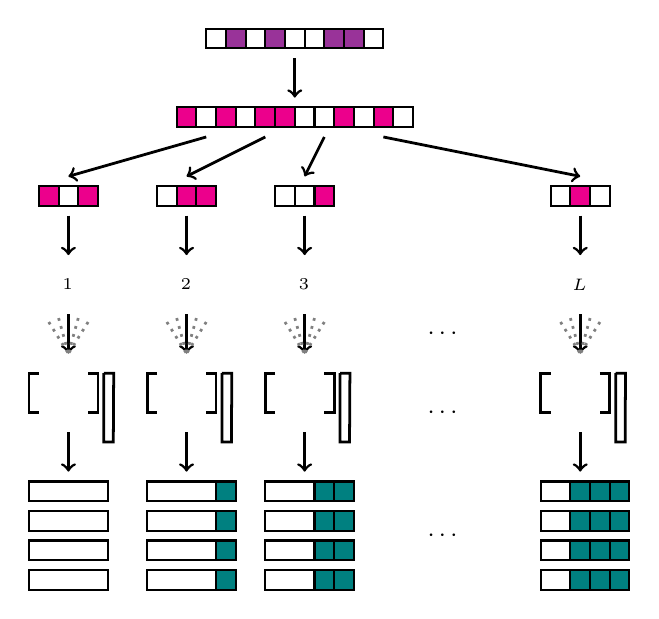
\begin{tikzpicture}
[font=\small, draw=black, line width=0.75pt,
sub0/.style={rectangle, draw, inner sep=0pt, minimum width=10mm, minimum height=2.5mm},
parity/.style={rectangle, draw, fill=teal, inner sep=0pt, minimum size=2.5mm},
bit0/.style={rectangle, draw, inner sep=0pt, minimum size=2.5mm},
bit1/.style={rectangle, draw, fill=violet!80, inner sep=0pt, minimum size=2.5mm},ebit0/.style={rectangle, draw, inner sep=0pt, minimum size=2.5mm},
ebit1/.style={rectangle, draw, fill=magenta, inner sep=0pt, minimum size=2.5mm}
]

\node[bit0] (info0) at (0.875,9.25) {};
\node[bit1] (info1) at (1.125,9.25) {};
\node[bit0] (info2) at (1.375,9.25) {};
\node[bit1] (info3) at (1.625,9.25) {};
\node[bit0] (info4) at (1.875,9.25) {};
\node[bit0] (info5) at (2.125,9.25) {};
\node[bit1] (info6) at (2.375,9.25) {};
\node[bit1] (info7) at (2.625,9.25) {};
\node[bit0] (info8) at (2.875,9.25) {};

\draw[->, line width=1pt]  (1.875,9) -- (1.875,8.5);

\node[ebit1] (bit0) at (0.50,8.25) {};
\node[ebit0] (bit1) at (0.75,8.25) {};
\node[ebit1] (bit2) at (1.00,8.25) {};
\node[ebit0] (bit3) at (1.25,8.25) {};
\node[ebit1] (bit4) at (1.50,8.25) {};
\node[ebit1] (bit5) at (1.75,8.25) {};
\node[ebit0] (bit6) at (2.00,8.25) {};
\node[ebit0] (bit7) at (2.25,8.25) {};
\node[ebit1] (bit8) at (2.50,8.25) {};
\node[ebit0] (bit9) at (2.75,8.25) {};
\node[ebit1] (bit10) at (3.00,8.25) {};
\node[ebit0] (bit11) at (3.25,8.25) {};

\draw[->, line width=1pt]  (0.75,8.00) -- (-1.00,7.50);
\draw[->, line width=1pt]  (1.50,8.00) -- (0.50,7.50);
\draw[->, line width=1pt]  (2.25,8.00) -- (2.00,7.50);
\draw[->, line width=1pt]  (3.00,8.00) -- (5.50,7.50);

\node[ebit1] (s00) at (-1.25,7.25) {};
\node[ebit0] (s01) at (-1.00,7.25) {};
\node[ebit1] (s02) at (-0.75,7.25) {};

\node[ebit0] (s03) at (0.25,7.25) {};
\node[ebit1] (s04) at (0.50,7.25) {};
\node[ebit1] (s05) at (0.75,7.25) {};

\node[ebit0] (s06) at (1.75,7.25) {};
\node[ebit0] (s07) at (2.00,7.25) {};
\node[ebit1] (s08) at (2.25,7.25) {};

\node[ebit0] (s09) at (5.25,7.25) {};
\node[ebit1] (s10) at (5.50,7.25) {};
\node[ebit0] (s11) at (5.75,7.25) {};

\draw[->, line width=1pt]  (-1.00,7) -- (-1.00,6.5);
\draw[->, line width=1pt]  (0.50,7) -- (0.50,6.5);
\draw[->, line width=1pt]  (2.00,7) -- (2.00,6.5);
\draw[->, line width=1pt]  (5.50,7) -- (5.50,6.5);

\node (cs1) at (-1.00,6.125) {$\xv_1$};
\node (cs2) at (0.50,6.125) {$\xv_2$};
\node (cs3) at (2.00,6.125) {$\xv_3$};
\node (cs4) at (5.50,6.125) {$\xv_L$};

\foreach \v in {-1.00,0.50,2.00,5.50} {
  \draw[->, line width=1pt]  (\v,4.25) -- (\v,3.75);
  \draw[->, line width=1pt]  (\v,5.75) -- (\v,5.25);
  \draw[dotted, line width=1pt, draw=gray]  (\v-0.25,5.65) -- (\v,5.25);
  \draw[dotted, line width=1pt, draw=gray]  (\v-0.125,5.7) -- (\v,5.25);
  \draw[dotted, line width=1pt, draw=gray]  (\v+0.125,5.7) -- (\v,5.25);
  \draw[dotted, line width=1pt, draw=gray]  (\v+0.25,5.65) -- (\v,5.25);
}

\node (dots1) at (3.75,5.5) {$\cdots$};

\foreach \v in {-1.00,0.50,2.00,5.50} {
  \draw[line width=1pt] (\v-0.375,5) -- (\v-0.5,5) -- (\v-0.5,4.5) -- (\v-0.375,4.5);
  \draw[line width=1pt] (\v+0.25,5) -- (\v+0.375,5) -- (\v+0.375,4.5) -- (\v+0.25,4.5);
  \draw[line width=1pt] (\v+0.45,5) -- (\v+0.45,4.125) -- (\v+0.57,4.125) -- (\v+0.575,5) -- (\v+0.45,5);
}

\node (dots2) at (3.75,4.5) {$\cdots$};
\node (dots3) at (3.75,2.9375) {$\cdots$};

\foreach \c in {3.50, 3.125, 2.75, 2.375} {
  \node[sub0] (subcs1\c) at (-1.00,\c) {};
  \node[sub0] (subcs2\c) at (0.50,\c) {};
  \node[sub0] (subcs3\c) at (2.00,\c) {};
  \node[sub0] (subcsL\c) at (5.50,\c) {};
}

\foreach \c in {3.50, 3.125, 2.75, 2.375} {
  \node[parity] (parity2\c) at (1,\c) {};
  \node[parity] (parity31\c) at (2.25,\c) {};
  \node[parity] (parity32\c) at (2.50,\c) {};
  \node[parity] (parityL1\c) at (5.5,\c) {};
  \node[parity] (parityL2\c) at (5.75,\c) {};
  \node[parity] (parityL3\c) at (6,\c) {};
}

\end{tikzpicture}
